\documentclass{article}
\usepackage[utf8]{inputenc}
\usepackage[margin=0.9in]{geometry}
\usepackage{titling}
\usepackage[utf8]{inputenc}
\usepackage[english]{babel}
\usepackage{amsthm}
\usepackage{amsmath}
\usepackage{amssymb}
\usepackage{graphicx}
\usepackage{changepage}
\usepackage{enumerate}

\graphicspath{ {/home/marko/Problem solving maths group} }
\newtheorem*{theorem}{Theorem}
\newtheorem*{definition}{Definition}
\newtheorem{example}{Example}
\newtheorem{exercise}{Exercise}

\title{\textbf{Computational Geometry}\\Shoelace formula and Convex Hull}
\date{Week 3}
\author{Marko Puza \\ Miroslav Stankovic}
\begin{document}
\maketitle

\section*{Shoelace formula}
The Shoelace formula provides a way to compute the area of any simple polygon given the coordinates of all vertices. Suppose we have a simple polygon with $n$ sides and vertices $(x_i, y_i); \ i = 1, \dots, n$. Then its area $A$ is: \[A = \frac{1}{2} |(x_1 y_2 + x_2 y_3 + \cdots + x_{n-1} y_n + x_n y_1)  - (x_2 y_1 + x_3 y_2 + \cdots + x_n y_{n-1} + x_1 y_n)|\]
or, equivalently:
\[A = \frac{1}{2}|\sum_{i=1}^n \det{\left( \begin{smallmatrix} x_i&x_{i+1}\\ y_i&y_{i+1} \end{smallmatrix} \right)}|\]
where $x_{n+1} = x_1, y_{n+1} = y_1$. \\\\
Where does the name of the formula come from? Let's try to use the formula on a trianlge with vertices in points $(2, 4), (3, -8), (1, 2)$. This gives us: $A = \frac{1}{2} | (2 \cdot (-8) + 3 \cdot 2 + 1 \cdot 4) - (4 \cdot 3 + (-8) \cdot 1 + 2 \cdot 2) | = 7$.

\begin{center}
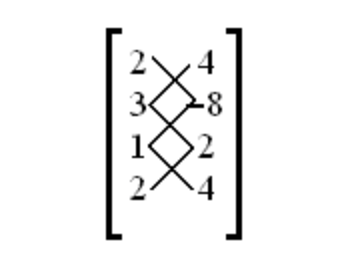
\includegraphics[width=4cm]{shoelace}
\end{center}

\begin{exercise}
    Show that the shoelace formula holds for any triangle.
\end{exercise}

\begin{exercise}
    Use this to prove that the shoelace formula holds for any convex polygon.
\end{exercise}

\noindent As a brief reminder from the last week, recall the Pick's formula.
\begin{theorem}[Pick's formula]
The area $A$ of a simple polygon with vertices in the grid points can be found as:
 \[A = i + \frac{b}{2} - 1\] where $i$ is the number of grid points in the interior of the polygon and $b$ the number of grid points on the polygon boundary. \\
\end{theorem}

\begin{exercise}
Most of the time, the computer programs estimate all shapes by polygons - thus both Pick's theorem and the Shoelace formula could be applied to estimate their areas. Can you think of simple algorithms for both? What is their efficiency?
\end{exercise}

\begin{exercise}
Given $n$ vertices of a simple polygon, devise an $\mathcal{O}(n)$ algorithm to find the number of integer points that are inside the polygon or on its boundary.
\end{exercise}

\section*{Convex hull}
Convex hulls are an ubiquitous concept in computational geometry, with an extensively long list of applications. Here, we will derive an efficient algorithm to find the convex hull - \textit{Graham scan}. \\\\
\noindent Let's start by recalling the definition of convexity.

\begin{definition}[Convexity]
A set of points $S$ is said to be \textit{convex} if for any two points $x, y$ in the set, the whole line segment $xy$ lies in the set.
\end{definition}

\begin{exercise}
Think of a few examples of convex sets in one, two and three dimensions. Is it necessary for a convex set to contain its boundary?
\end{exercise}

\noindent From now one, we will, however, only consider the convex sets that contain its boundary\footnote{such sets are called closed}. We can formally define the convex hull of a set of points as:

\begin{definition}[Convex hull]
Convex hull of a set of points $S$ is the intersection of all half-spaces that contain $S$.
\end{definition}

\noindent Note here, that by half-space in 1 dimension we mean the set of points lying on one side of the point, in 2 dimensions the set of points lying on one side of the line and so on. Suppose that we are given some finite number of points on a plane - if we imagine these points as being nails on a board, the convex hull is just a polygon that will be formed when we put an elastic band around all the nails.

\begin{center}
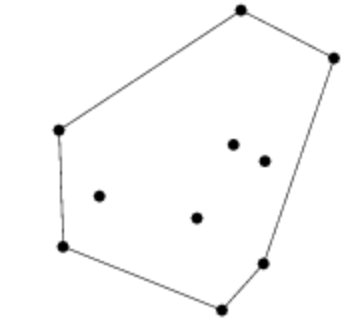
\includegraphics[width=4cm]{hull}
\end{center}

\noindent As a few examples where it is very useful to be able to compute the convex hull efficiently, we can mention the robot motion planning in robotics, the collision detection in computer games or a general method called \textit{convex relaxation} in optimisation problems (often it is much easier to solve convex problems, and convex hull provides a convex approximation).

\begin{exercise}
What are the ways that the convex hull may be used in robot motion planning or collision detection?
\end{exercise}

\begin{exercise}
Try to think of a simple way to compute/find the convex hull, given set of points.
\end{exercise}

\section*{Graham scan}
The Graham scan consists of the following steps:

\begin{enumerate}[(i)]
    \item {
        Choose the point $P$ with the smallest $y$-coordinate (and the smallest $x$-coordinate in case of ties).
    }
    \item {
        Sort the points increasingly by the angle that they and point $P$ make with the $x$-axis.
    }
    \item {
        Consider now the hull as being only $H = \{P\}$ and start adding points in this sorted order. When a point $Q$ is added, look if we need to make a right-turn or a left-turn with respect to the last two points in the hull. If it is a left-turn, point $Q$ is in the hull and we can continue. If it is a right-turn, keep removing the points preceding $Q$ from the hull until the turn that we are making is a left-turn.
    }
    \item {
        Once we reach point $P$ again, $H$ will contain precisely the points that form the convex hull, in counterclockwise order.
    }

\end{enumerate}

\break

\begin{exercise}
Try to go through the Graham scan on some set of points, using pen and paper.
\end{exercise}

\begin{exercise}
What is the time efficiency of the Graham scan? (You can use the fact that sorting takes $\mathcal{O}(n \log{n})$ time).
\end{exercise}

\begin{exercise}
Show that a point p in S is a vertex of the convex hull if and only if there is a line going through p such that all the other points in S are on the same side of the line.
\end{exercise}

\begin{exercise}
Given two convex polygons represented by their vertices, design an algorithm to check if one polygon is completely contained within the second one.
\end{exercise}

\begin{exercise}
Suppose we have a convex hull of a set of points. We will add one other point to the set of points - how can we find the new convex hull in $\mathcal{O}(n)$ time?
\end{exercise}

\begin{exercise}[The bomb problem]
Given $n$ points in a plane, find the smallest circle that contains all of the points in $\mathcal{O}(n^4)$ time. Can we do better? (the best know result is $\mathcal{O}(n)$).
\end{exercise}

\begin{exercise}
What would go wrong with the Graham scan in three dimensions?
\end{exercise}

\end{document}
